
\newpage
\section{Appendix}



\subsection{Judge Model Analysis}
\label{app:judge_model}
We analyze the judge model's performance on the labeled validation set. 
We compare \GraphEval{}'s judge model by using the last token logit as the judge model. This is a common practice in evaluating LLMs, as the last token logit is the most common way to extract the hidden state of the LLMs. We also analyze the judge model with or without the prompt encoder (PE), as it may have a negative impact on the judge model's performance. We refer to Figure~\ref{fig:evaluation_scores} for the judge model's performance on the labeled validation set. 


\begin{figure}[t]
\captionsetup[subfloat]{aboveskip=1pt,belowskip=1pt}
    \centering
    
\includegraphics[width=5.5in]{submissions/Jing2024/figures/experiments/evaluation_scores/legend_abla.pdf}\\
     \vspace{-5mm}
    \subfloat[LLaMA 7B]{
        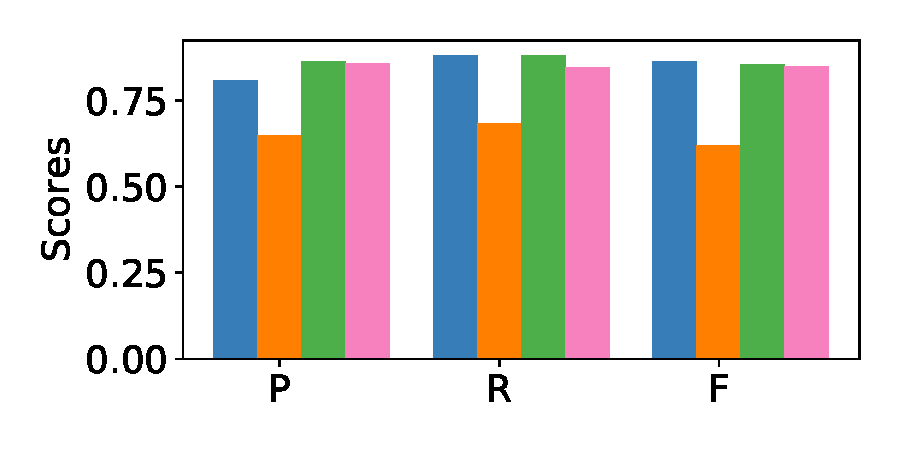
\includegraphics[width=1.78in]{submissions/Jing2024/figures/experiments/evaluation_scores/evaluation_scores_llama_2_7b.pdf}
        \label{fig:evaluation_scores_llama_2_7b}
       }\hspace{-4mm}
    \subfloat[LLaMA 13B]{
        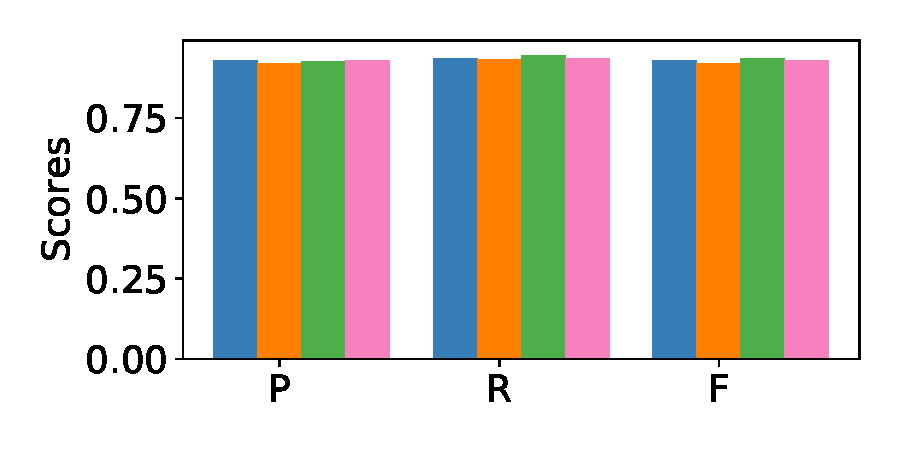
\includegraphics[width=1.78in]{submissions/Jing2024/figures/experiments/evaluation_scores/evaluation_scores_llama_2_13b.pdf}
        \label{fig:evaluation_scores_llama_2_13b}
       }\hspace{-4mm}
    \subfloat[LLaMA 70B]{
        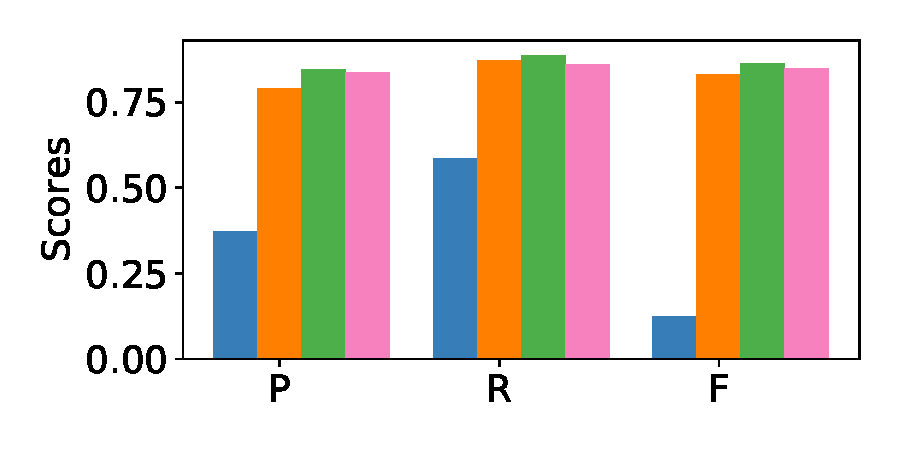
\includegraphics[width=1.78in]{submissions/Jing2024/figures/experiments/evaluation_scores/evaluation_scores_llama_2_70b.pdf}
        \label{fig:evaluation_scores_llama_2_70b}
       }
    \\\vspace{-4mm}
    \subfloat[Gemma 2B]{
        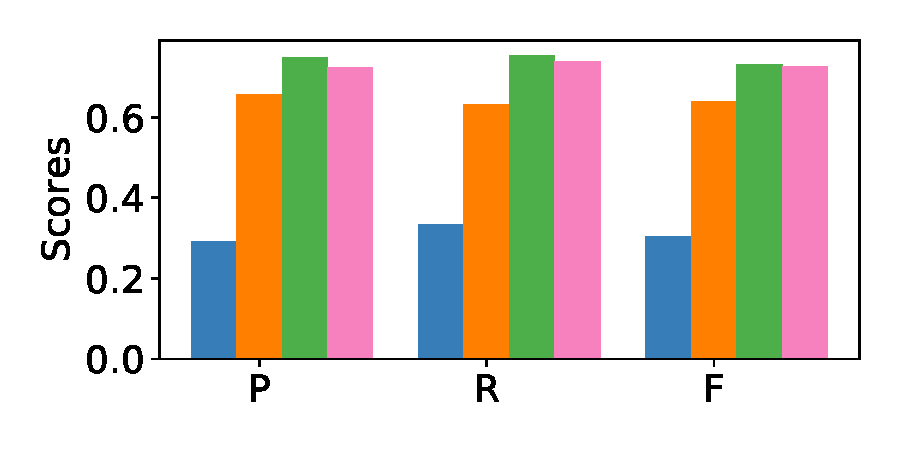
\includegraphics[width=1.78in]{submissions/Jing2024/figures/experiments/evaluation_scores/evaluation_scores_gemma_2b.pdf}
        \label{fig:evaluation_scores_gemma_2b}
       }\hspace{-4mm}
    \subfloat[Gemma 7B]{
        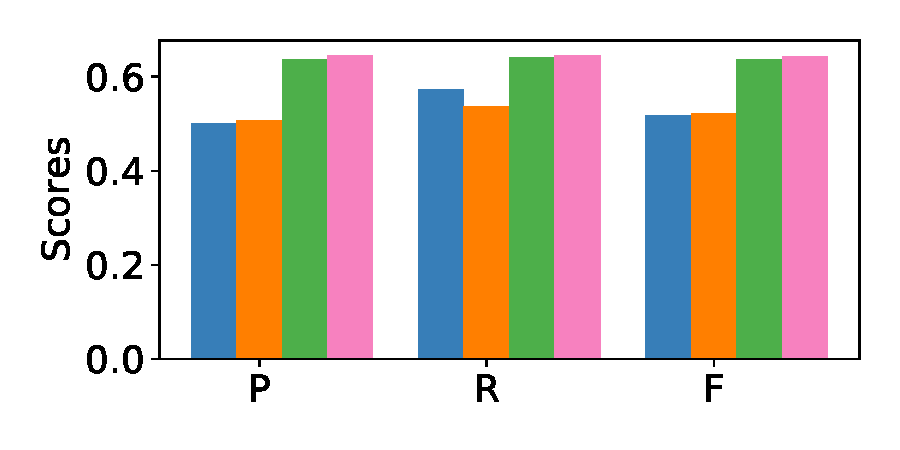
\includegraphics[width=1.78in]{submissions/Jing2024/figures/experiments/evaluation_scores/evaluation_scores_gemma_7b.pdf}
        \label{fig:evaluation_scores_gemma_7b}
       }\hspace{-4mm}
    \subfloat[Average]{
        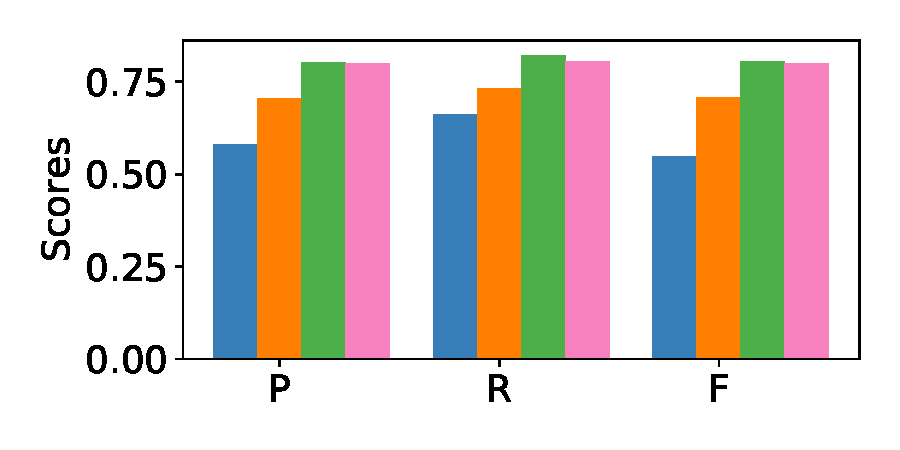
\includegraphics[width=1.78in]{submissions/Jing2024/figures/experiments/evaluation_scores/evaluation_scores_average.pdf}
        \label{fig:evaluation_scores_average}
       }
       \vspace{-3mm}
    \caption{Evaluation scores on the judge model's performance on the labeled validation set. P, R, and F are Precision, Recall, and F1 Score. 
    }
    \vspace{-3mm}
    \label{fig:evaluation_scores}
\end{figure}


\begin{table}[t]
    \centering
    \setlength{\tabcolsep}{2mm}{
    \begin{tabular}{lcccccccccc}
    \toprule
    \multirow{2}{*}{\textbf{Substitute Model}}  & \multicolumn{3}{c}{\textbf{LLaMA 2 7B}} & \multicolumn{3}{c}{\textbf{LLaMA 2 13B}} & \multicolumn{3}{c}{\textbf{LLaMA 2 70B}} \\
    \cmidrule(lr){2-4} \cmidrule(lr){5-7} \cmidrule(lr){8-10} 
    
    & P & R & F & P & R & F & P & R & F  \\
    \midrule
    \textbf{LLaMA 2 7B} & .858 & .845 & .850 & .928 & .934 & .930 & .837 & .861 & .848 \\
    \textbf{LLaMA 2 13B} & .850 & .868 & .855 & .930 & .940 & .932 & .837 & .851 & .844 \\
    \textbf{LLaMA 2 70B} & .868 & .883 & .871 & .924 & .942 & .931 & .858 & .876 & .866 \\
 
    \bottomrule
    \end{tabular}}
    \caption{Ablation on the LLaMA models as substitute models. The $i$-th row and $j$-th column denote the result of using $i$-th LLM as the substitute hidden state input for training on $j$-th model's labels.  P, R, and F are Precision, Recall, and F1 Score.  
    }
    \label{tab:abla_substitute}
    \end{table}


    






\begin{table}[t]
    \centering
    \small
    \setlength{\tabcolsep}{.5mm}{
    \begin{tabular}{lcccccccccc}
    \toprule
    \multirow{2}{*}{\textbf{Models}}
    & \multicolumn{2}{c}{\textbf{LLaMA 2 7B}} & \multicolumn{2}{c}{\textbf{LLaMA 2 13B}} & \multicolumn{2}{c}{\textbf{LLaMA 2 70B}} & \multicolumn{2}{c}{\textbf{Gemma 2B}} & \multicolumn{2}{c}{\textbf{Gemma7B}} \\
    \cmidrule(lr){2-3} \cmidrule(lr){4-5} \cmidrule(lr){6-7} \cmidrule(lr){8-9} \cmidrule(lr){10-11}
      & Speed & \#GPUs   & Speed & \#GPUs  & Speed & \#GPUs & Speed & \#GPUs & Speed & \#GPUs \\
    \midrule
    TG (A6000) & 2.26 & 1 & 1.07 & 2 & 0.09 & 4 & 2.06 (1.82) & 1 & 2.18 (1.28) & 1 \\
    \GraphEval{} (A6000) & 121.34  & 1 & 120.10 & 1 & 117.90 & 1 & 388.61 & 1 & 389.04 & 1 \\
    \midrule
    TG (A100) &  2.80 & 1 & 1.48 & 1 & 0.21 & 2 & 2.47 & 1 & 2.42 & 1 \\
    \GraphEval{} (A100) &  210.59 & 1 & 213.05 & 1 & 210.30 & 1 & 731.98 & 1 & 735.62 & 1 \\
    \bottomrule
    \end{tabular}}
    \caption{Efficiency evaluation. Speed denotes the average number of triple facts on which a conclusion can be given in one second. \#GPUs denotes the least number of GPUs to run without OOM. TG denotes text generation. 
     The numbers in parentheses are the speed without Flash Attention 2.}
    \label{tab:speed_test}
\end{table}

    


 \paragraph{Accuracy Analysis}
 The  \GraphEval{} model, both with and without Prompt Encoder (PE), consistently outperforms the score of using Last token logits in almost all configurations and metrics. This indicates the effectiveness of the  \GraphEval{} approach in capturing the nuances of the evaluation task.

 \paragraph{Ablation Study}
{\it On Prompt Encoder:}
As Figure~\ref{fig:evaluation_scores} shows, 
the comparison between models with and without PE indicates a slight performance variation. For \GraphEval{}, the presence of PE does not significantly alter the performance, suggesting that our method of evaluating LLMs is robust to the inclusion or exclusion of PE.
For the Last token logits method, removing PE generally results in a perturbation in performance. However, the  \GraphEval{} approach's consistency suggests a potentially different or more advanced mechanism of evaluation that is less dependent on PE.
{\it On Substitute Models:}
We also evaluate the judge model's performance on different LLMs as hidden state input. 
We refer to Table \ref{tab:abla_substitute} for the judge model's performance on different LLMs as hidden state input. We can see that, generally, when larger models are applied for feeding the hidden states, there is a slight increase in the fitting accuracy of the judge model. However, there is no significant difference in the judge model's performance.



\paragraph{Efficiency study}
We also analyze the judge model's efficiency by measuring the time it takes to make a prediction on one triple.
The speed of text generation refers to the average rate at which the LLM completes generating a response consisting of one sentence derived from a triple. It's important to recognize that the pace of text generation can vary with different prompts because the LLM may produce responses of varying lengths. Therefore, for a more consistent measure of text generation speeds, it's advisable to consider the rate of token generation. Despite this, our evaluation framework, \GraphEval{}, does not depend on text generation and operates on a triple-based unit. Consequently, we continue to use the triple as the unit of measurement for time.
We use the same hardware and software environment for all the experiments. We compare the average speed of the judge model with text generation. We report the time it takes to make a prediction in Table \ref{tab:speed_test}. 
 The attention implementation and precision are the same for text generation and for the judge model's input model. 
 We can see that the judge model is significantly faster than text generation. This indicates that the judge model is efficient in evaluating the LLMs. Also, benefiting from the substitute model, our evaluation speed and GPU requirement does not grow with the LLM size, which is an advantage for evaluating large LLMs.
 We also observe that, paradoxically, the Gemma 2B model operates slower than the Gemma 7B model, despite its smaller size. This counterintuitive result could be attributed to the implementation of Flash Attention 2. To draw a fair comparison, we documented the text generation speed on A6000 GPUs excluding Flash Attention 2, which is indicated within parentheses. The comparative data reveals that Gemma 2B is faster than Gemma 7B when Flash Attention 2 is not utilized. Notwithstanding this, Gemma 2B demonstrates enhanced performance when Flash Attention 2 is active. Therefore, for the sake of consistency, we have decided to maintain the results acquired with Flash Attention 2.


\subsection{Detailed Relation Type Analysis}
\label{app:relation_type_study}




\begin{figure}[t]
\centering
 
\includegraphics[width=6in]{submissions/Jing2024/figures/experiments/relation_analysis/legend.pdf}
\\\vspace{-6mm}
\subfloat[\textit{Correctness} vs Head entity type]{
 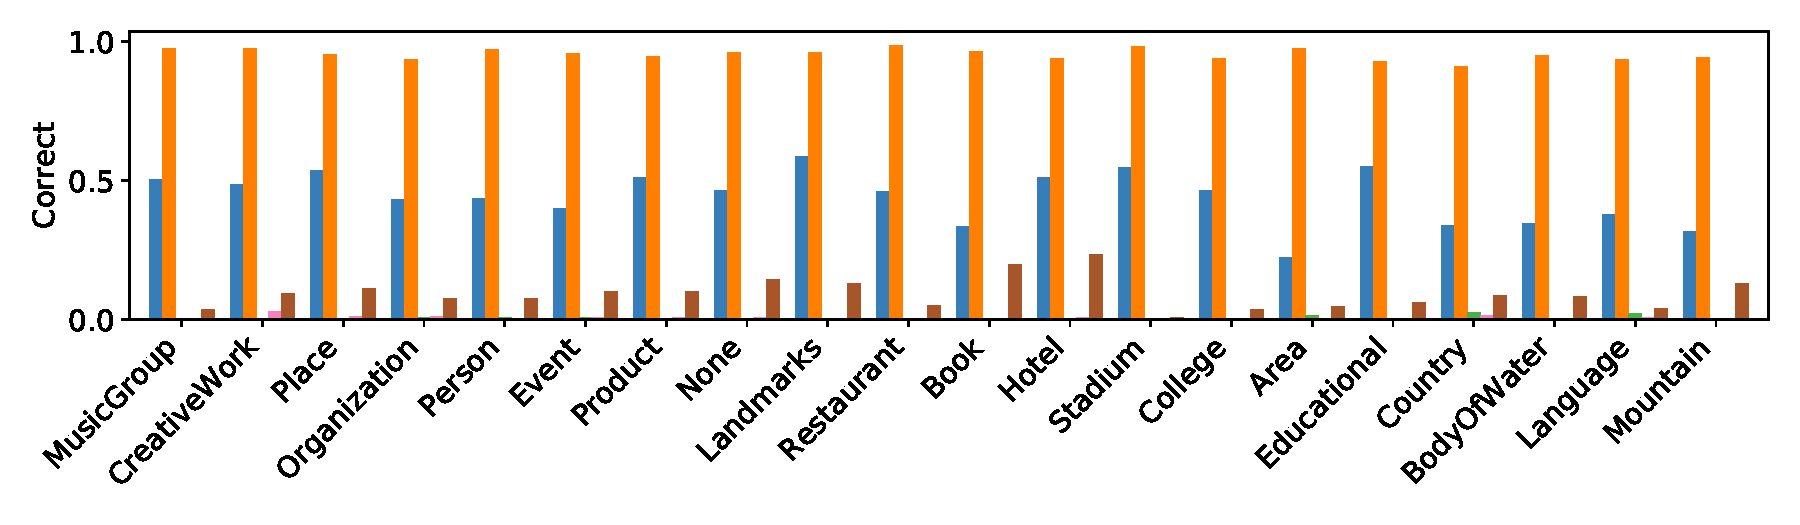
\includegraphics[width=5.5in]{submissions/Jing2024/figures/experiments/relation_analysis/correct_by_head_type.pdf}
 \label{fig:correct_by_head_type}
}\\

\includegraphics[width=5.5in]{submissions/Jing2024/figures/experiments/relation_analysis/legend.pdf}
\\\vspace{-6mm}
\subfloat[\textit{Correctness} vs Tail entity type]{
 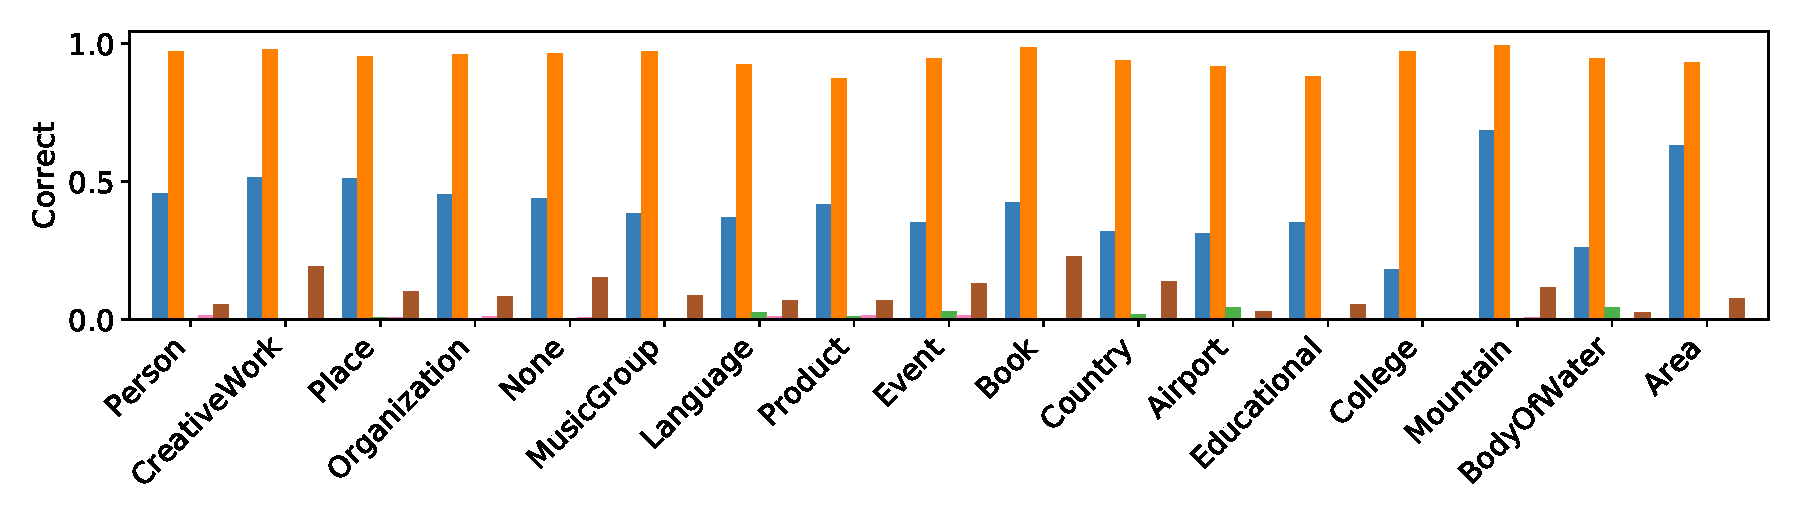
\includegraphics[width=5.5in]{submissions/Jing2024/figures/experiments/relation_analysis/correct_by_tail_type.pdf}
 \label{fig:correct_by_tail_type}
}
\caption{The LLM's \textit{correctness} with respect to head entity types and tail entity types}
\label{fig:correctness_by_type}
\end{figure}


\begin{figure}[t]
    \centering
 
\includegraphics[width=5.5in]{submissions/Jing2024/figures/experiments/relation_analysis/legend.pdf}
 \\\vspace{-6mm}
\subfloat[\textit{Truthfulness} vs Head entity type]{
 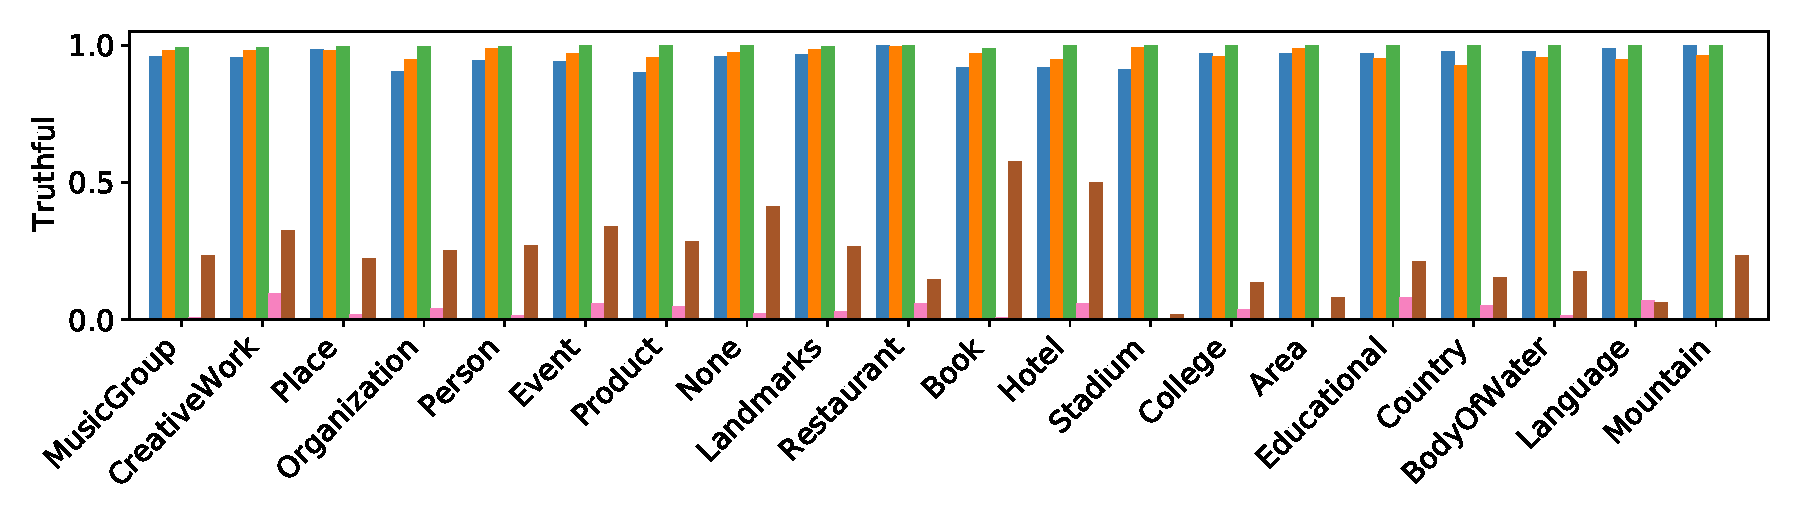
\includegraphics[width=5.5in]{submissions/Jing2024/figures/experiments/relation_analysis/truthful_by_head_type.pdf}
 \label{fig:truthful_by_head_type}
}\\

\includegraphics[width=5.5in]{submissions/Jing2024/figures/experiments/relation_analysis/legend.pdf}
\\\vspace{-6mm}
\subfloat[\textit{Truthfulness} vs Tail entity type]{
 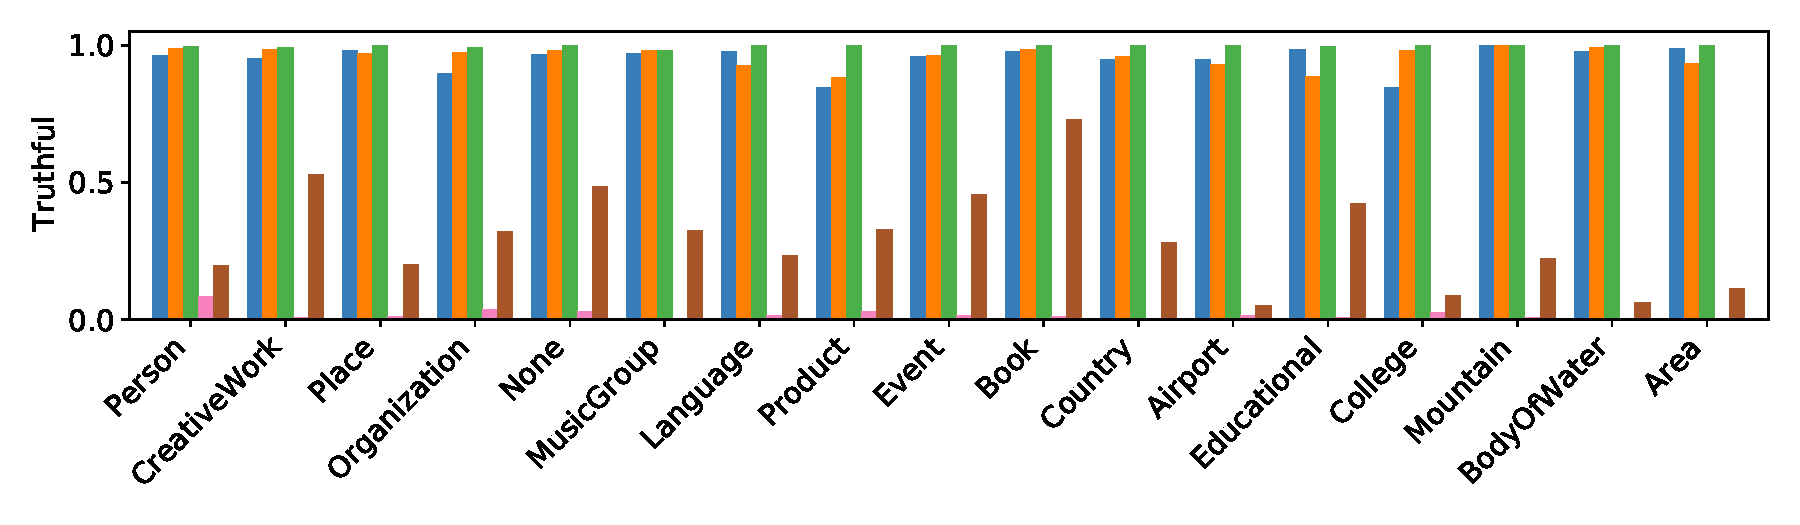
\includegraphics[width=5.5in]{submissions/Jing2024/figures/experiments/relation_analysis/truthful_by_tail_type.pdf}
 \label{fig:truthful_by_tail_type}
}
\caption{The LLM's \textit{truthfulness} with respect to head entity types and tail entity types}
\label{fig:truthfulness_by_type}
\end{figure}
\begin{figure}[t]
    \centering
    
\includegraphics[width=6in]{submissions/Jing2024/figures/experiments/relation_analysis/legend.pdf}
    \\\vspace{-6mm}
\subfloat[\textit{Informativeness} vs Head entity type]{
 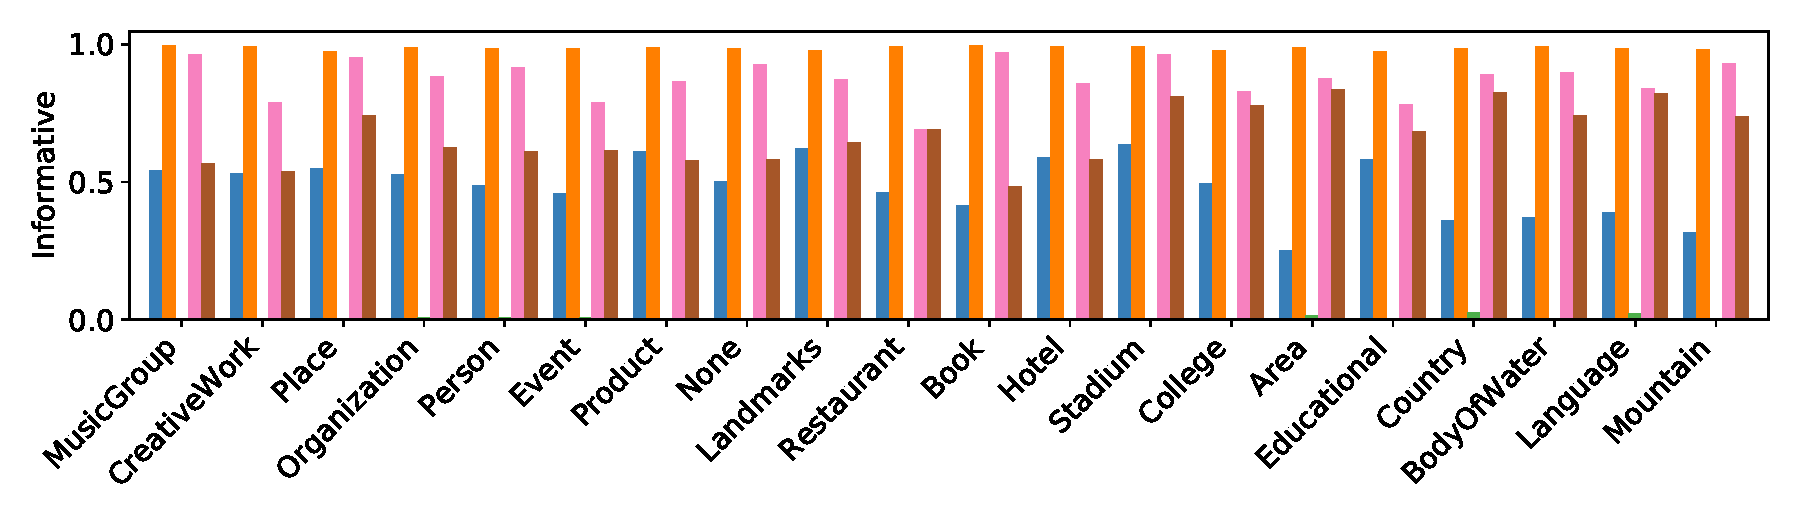
\includegraphics[width=5.5in]{submissions/Jing2024/figures/experiments/relation_analysis/informative_by_head_type.pdf}
 \label{fig:informative_by_head_type}
}\\

\includegraphics[width=5.5in]{submissions/Jing2024/figures/experiments/relation_analysis/legend.pdf}
\\\vspace{-6mm}
\subfloat[\textit{Informativeness} vs Tail entity type]{
 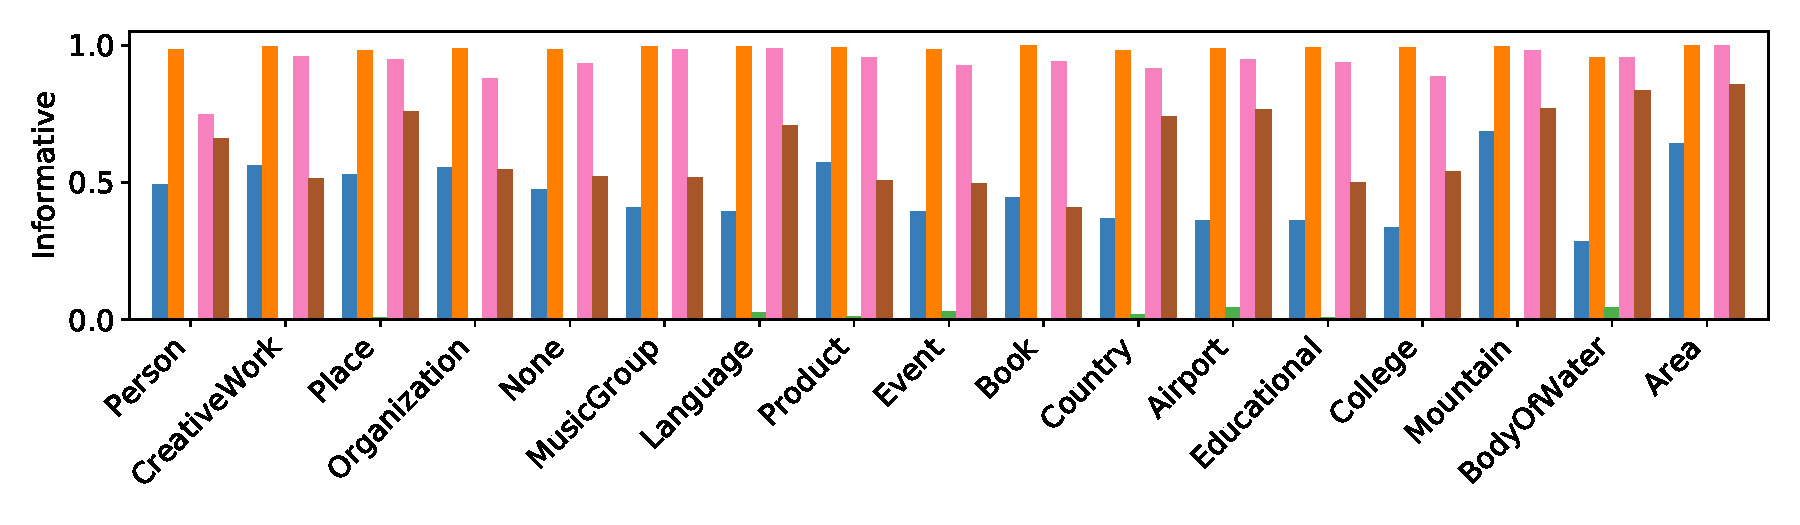
\includegraphics[width=5.5in]{submissions/Jing2024/figures/experiments/relation_analysis/informative_by_tail_type.pdf}
 \label{fig:informative_by_tail_type}
}
\caption{The LLM's \textit{informativeness} with respect to head entity types and tail entity types}
\label{fig:informativeness_by_type}
\end{figure}



\paragraph{Llama Family Analysis}
Across the LLaMA family, a progressive improvement in performance is observed from  7b to 13b. The 7b model shows decent performance across categories with a particular strength in the \textit{truthfulness}. However, its \textit{informativeness} and \textit{correctness} metrics show room for improvement, particularly in categories like Book, Hotel, and College, indicating a struggle to accurately provide informative and correct classifications in more nuanced or specific domains.

The LLaMA 13b model demonstrates a significant leap in performance, especially in \textit{informativeness} and \textit{correctness}, nearly reaching perfection across most categories. This jump can be attributed to the model's increased capacity, enabling it to understand and process the nuances of various entities better, resulting in remarkably high scores in nearly all categories, especially noticeable in MusicGroup, CreativeWork, and Place.

The LLaMA 70b results appear anomalous with extremely high \textit{truthfulness} scores but negligible \textit{informativeness} and \textit{correctness} across all categories. We suspect this discrepancy might be due to the model's knowledge awareness~\cite{ren2023investigating}, where the model might be less confident in its responses when the parameters are increased, leading to a higher proportion of ``I don't know" responses. This could explain the high \textit{truthfulness} scores but low \textit{informativeness} and \textit{correctness} metrics, as the model might be too cautious to provide definitive answers.

\paragraph{Gemma Family Analysis}
The Gemma models present an interesting contrast. The Gemma 2b model shows a tendency towards high \textit{informativeness} in certain categories like MusicGroup and Book but lacks behind significantly in \textit{truthfulness} and \textit{correctness} metrics. This suggests that while the model might be picking up on relevant information, it struggles to accurately validate the truth behind that information or its applicability to the queried entities.
The Gemma 7b model shows improvement in the \textit{truthfulness} metric compared to Gemma 2b, particularly noticeable in categories like Book and Hotel, and even surpasses LLaMA 7b in certain areas like None and Restaurant. However, it still significantly lags behind the LLaMA models, particularly LLaMA 13b, in both \textit{informativeness} and \textit{correctness}. The improved but still limited performance suggests that while Gemma 7b has a better grasp over the veracity of information compared to Gemma 2b, it still struggles with providing highly informative and correct outputs consistently across various entities.



\subsection{Correlation Analysis}
\label{app:correlation_analysis}
As the current language models are all exposed to Wikipedia knowledge during training, we are interested in how the LLM performance is correlated with the attributes of the triples in the knowledge graphs. As an example, if an entity has a higher degree, it may be linked to more documents, and the LLM may have more chances to learn about the entity during training. Another example is the popularity of the entity. If the entity is more popular, it may be linked to more external documents \wfj{because it summarizes the relevant knowledge and provides high-level ideas to the general public}, and the LLM may have more chances to learn about the entity during training. This raises the question of whether the LLM's performance is correlated with the attributes of the triples in the knowledge graphs.
For the entities in a knowledge graph, the degree of an entity is the number of edges connected to the entity. We also collect the \textit{pageviews} of the entities in the knowledge graph from Wikimedia\footnote{https://wikimedia.org/api/rest\_v1/metrics/pageviews/per-article/en.wikipedia.org/all-access/all-agents}{}, which is the number of pageviews of the Wikipedia page of the entity. This can be seen as a measure of the popularity of the entity  \wfj{because a popular page should appeal to the significant attention of the readers}. We collect the pageviews, in the time period of the entities in the knowledge graph from the Wikipedia page of the entity.
After collecting the degree and pageviews of the entities in the knowledge graph, we can aggregate the degree and pageviews of the entities to the triples, by simply taking the average of the degree and pageviews of the head and tail entities of the triples.

Here, we analyze whether the LLM's performance is correlated with the attributes of the triples in the knowledge graphs, such as the entity's degree, and page views. 
We refer to Figure \ref{fig:correlation_heatmap} for the correlation heatmap of the LLMs' hidden states and the judge model's predictions. Here, `T' stands for \textit{Truthful}, `I' stands for \textit{Informativeness}, `C' stands for \textit{Correctness}, `P' stands for Pageviews, and `D' stands for Degree. 
 We can see that the LLM's performance does not show a strong correlation with the attributes of the triples in the knowledge graphs. This indicates that the LLM's performance is not directly correlated with the attributes of the triples in the knowledge graphs. However, the different metrics of LLMs may correlate with each other, such as \textit{Truthful} and \textit{Informativeness}, which is expected. 
\xzrevision{This can be explained by the fact that certain attributes, like the degree of an entity in the knowledge graph, can be misleading. For example, degree is often correlated with popularity, but the popularity metric is 0 for many entities, particularly those in the long tail. This uneven distribution limits the usefulness of popularity as a reliable metric for evaluating LLM performance. In other words, while high-degree or popular entities may influence LLM performance to some extent, the vast majority of entities are long-tail, and their sparse or zero popularity values do not strongly correlate with performance outcomes. This highlights the need for more nuanced or domain-specific metrics to assess LLM performance effectively.}

\begin{figure}[t]
\centering
\subfloat[LLaMA-2-7B]{
 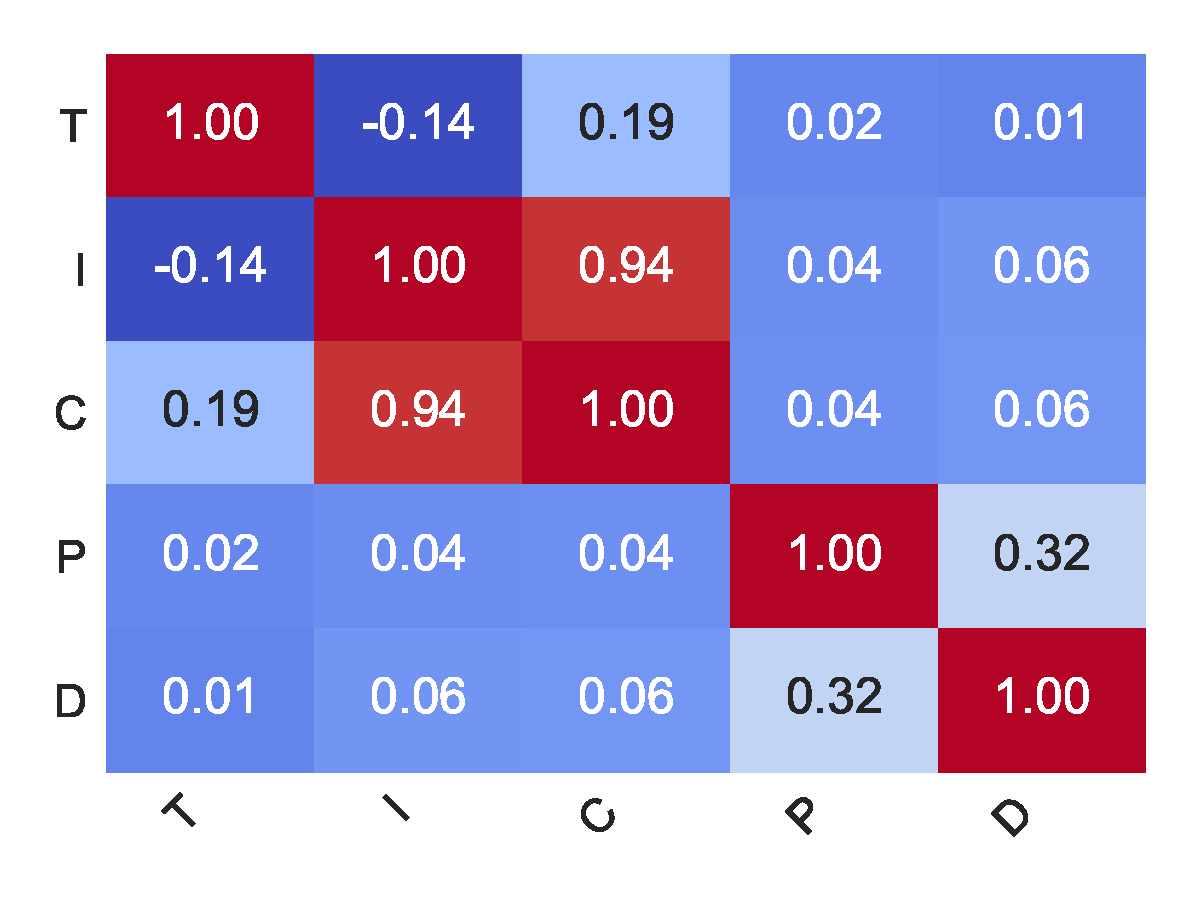
\includegraphics[width=1.6in]{submissions/Jing2024/figures/experiments/correlation_heatmap/correlation_heatmap_llama_7b.pdf}
 \label{fig:correlation_heatmap_llama_7b}
} 
\subfloat[LLaMA-2-13B]{
 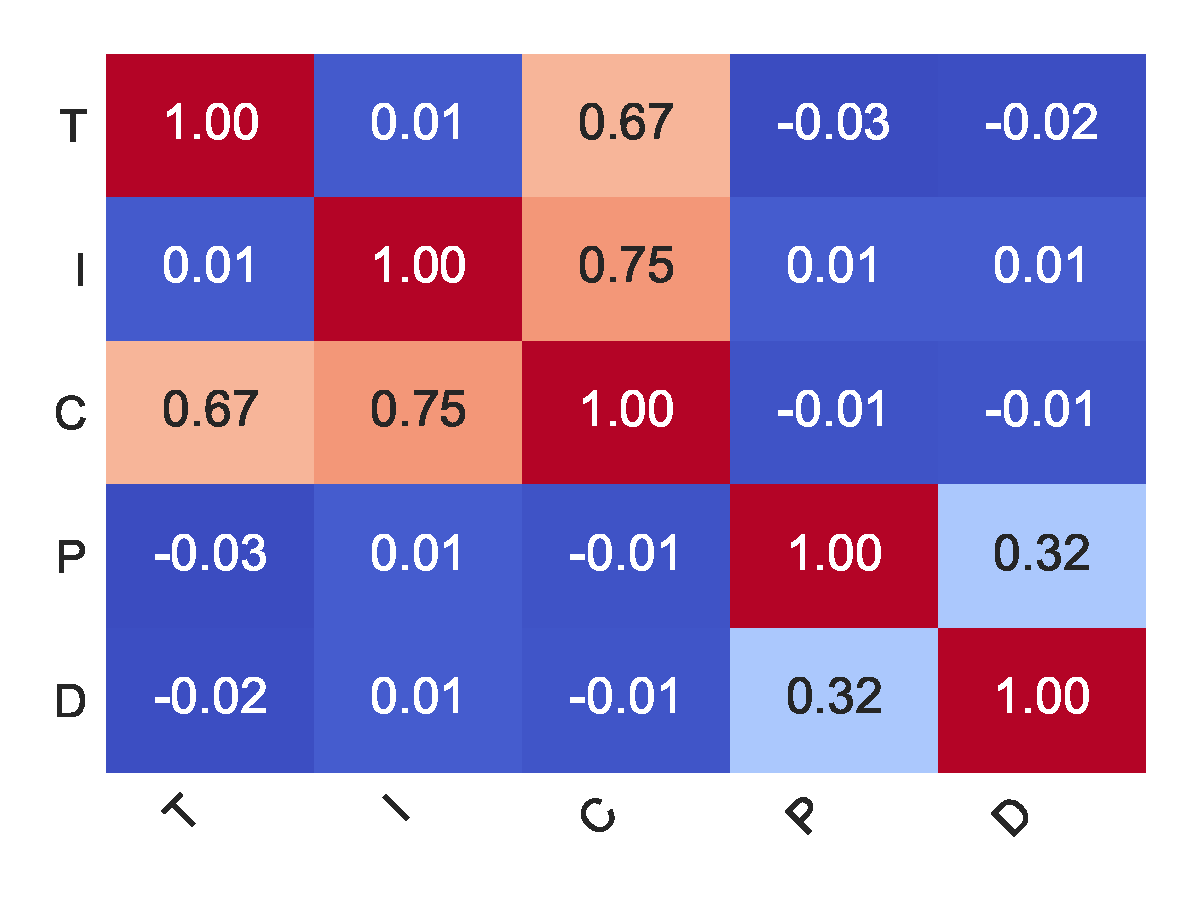
\includegraphics[width=1.6in]{submissions/Jing2024/figures/experiments/correlation_heatmap/correlation_heatmap_llama_13b.pdf}
 \label{fig:correlation_heatmap_llama_13b}
} 
\subfloat[LLaMA-2-70B]{
 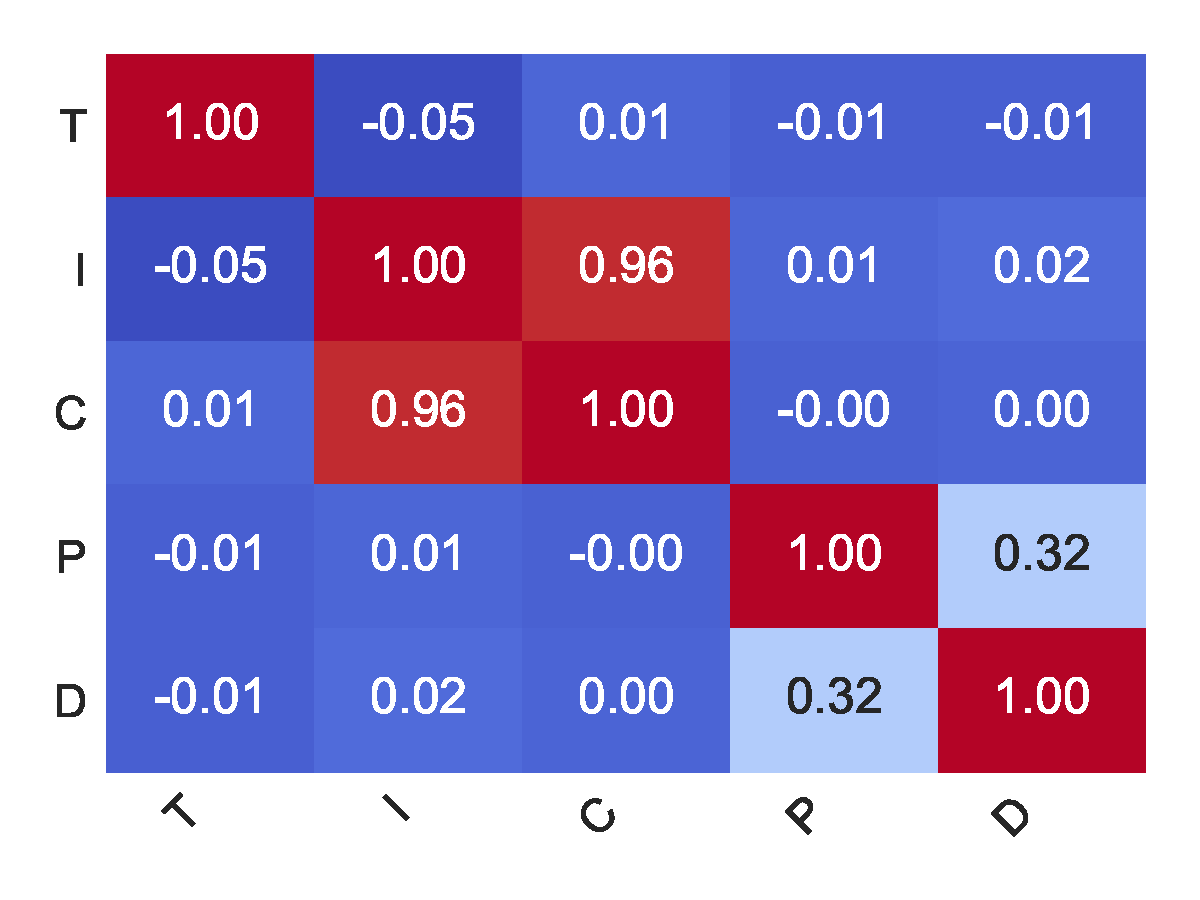
\includegraphics[width=1.6in]{submissions/Jing2024/figures/experiments/correlation_heatmap/correlation_heatmap_llama_70b.pdf}
 \label{fig:correlation_heatmap_llama_70b}
}
\\
\subfloat[Gemma-2B]{
 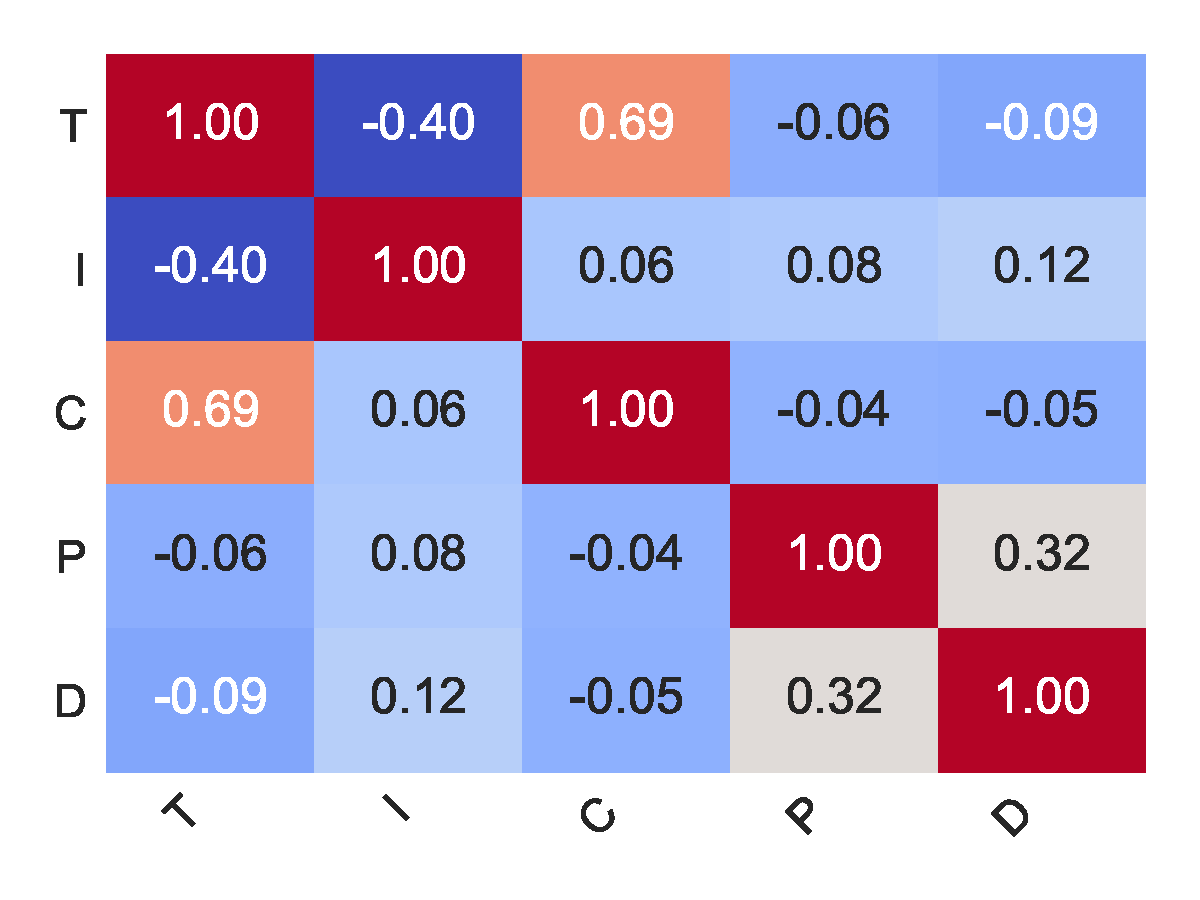
\includegraphics[width=1.7in]{submissions/Jing2024/figures/experiments/correlation_heatmap/correlation_heatmap_gemma_2b.pdf}
 \label{fig:correlation_heatmap_gemma_2b}
}
\subfloat[Gemma-7B]{
 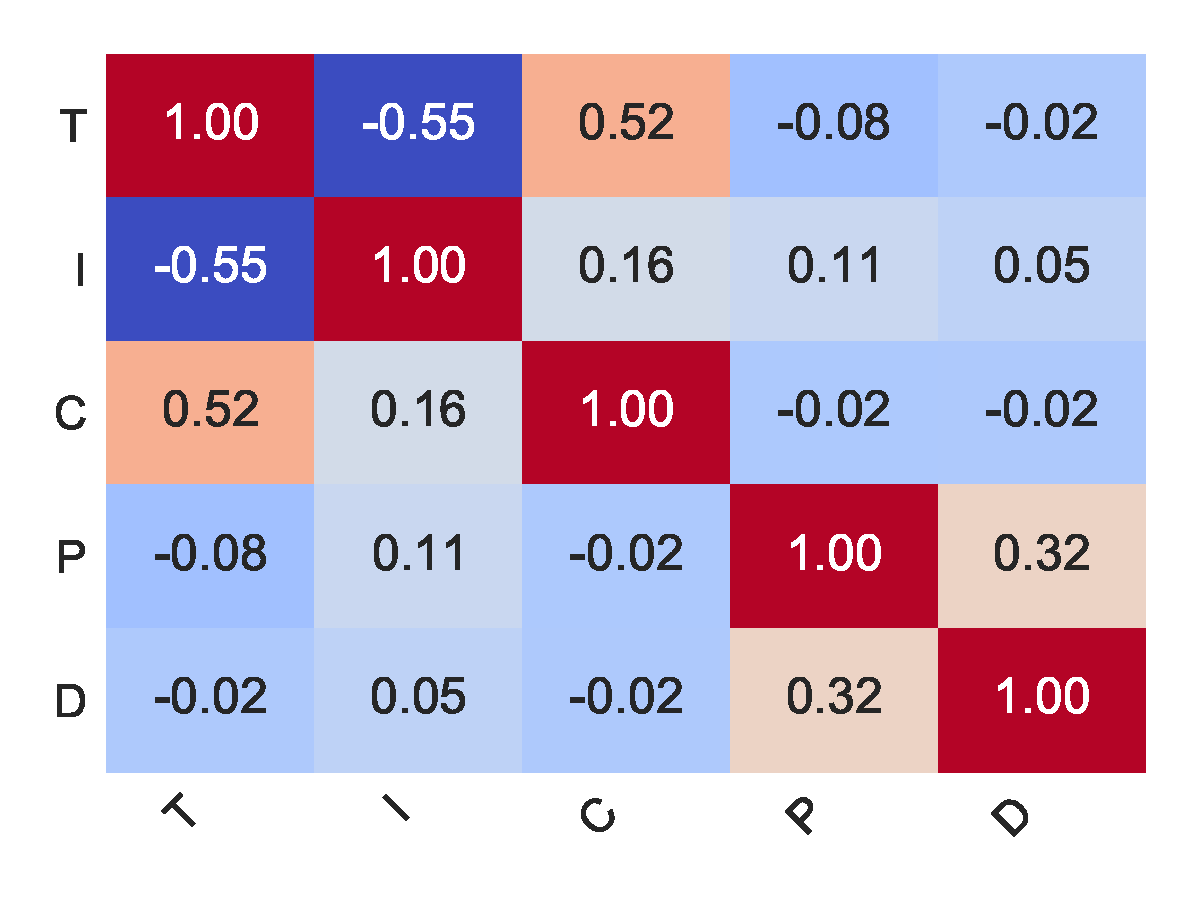
\includegraphics[width=1.7in]{submissions/Jing2024/figures/experiments/correlation_heatmap/correlation_heatmap_gemma_7b.pdf}
 \label{fig:correlation_heatmap_gemma_7b}
}
\caption{Correlation heatmap of the LLMs' hidden states and the judge model's predictions.}
\label{fig:correlation_heatmap}
\end{figure}





\subsection{Knowledge Boundary Analysis}\label{app:knowledge_boundary}

\subsection{Knowledge Boundary Analysis}\label{app:knowledge_boundary}

\subsection{Knowledge Boundary Analysis}\label{app:knowledge_boundary}
\input{submissions/Jing2024/src/tables/knowledge_boundary}
\xzrevision{We analyze the knowledge boundaries of large language models (LLMs), as discussed in Section \ref{sub:performance_analysis} and \cite{ren2023investigating}, which suggest that larger models have a better understanding whether they know an answer or not. To investigate this hypothesis, we conduct experiments using the Llama 3 model series on two question-answering datasets: CommonsenseQA \cite{CommonsenseQA} and TruthfulQA \cite{TruthfulQA}. To assess whether an LLM understands its own knowledge boundaries, we directly elicit confidence scores for each answer through prompting, then we calculate the Expected Calibration Error (ECE). ECE measures the misalignment between the correctness of answers and the models' confidence. Mathematically, for LLM responses $\mathcal{A}$, ECE is defined as:}

\begin{equation} \text{ECE} = \frac{1}{|\mathcal{A}|}\sum_{a\in\mathcal{A}} \left|\mathbb{I}(a) - \text{conf}(a)\right|, \end{equation}

\xzrevision{where $\mathbb{I}(a)$ is an indicator function that outputs 1 if $a$ is correct and 0 otherwise, and $\text{conf}(a)$ denotes the confidence score assigned by the model. The experimental results are presented in Table \ref{tab:ece_results}.}

\xzrevision{The results in Table \ref{tab:ece_results} align with our previous hypothesis across different Llama 3 model sizes. For both CommonsenseQA and TruthfulQA, the ECE values decrease as model size increases, indicating better alignment between confidence and correctness in larger models. Specifically, for CommonsenseQA, the Llama 3 70B model achieves the lowest ECE (22.28\%), demonstrating superior calibration compared to smaller models like Llama 3 1B (54.65\%). Similarly, on TruthfulQA, the Llama 3 70B model achieves an ECE of 23.45\%, significantly outperforming the smaller Llama 3 1B model with an ECE of 58.35\%.}

\xzrevision{These findings align with the hypothesis that larger models are better calibrated in estimating their confidence, which can partially explain why larger models are more likely to answer ``I don't know'' when asked about a question as shown in Section \ref{sub:performance_analysis}.}

\xzrevision{Overall, \GraphEval{} aligns well with the results on TruthfulQA and CommonsenseQA, demonstrating that it effectively captures the model's factuality and informativeness across diverse knowledge domains. This alignment validates the robustness of our evaluation framework and confirms its consistency with established benchmarks for assessing LLM reasoning and truthfulness. }


\xzrevision{We analyze the knowledge boundaries of large language models (LLMs), as discussed in Section \ref{sub:performance_analysis} and \cite{ren2023investigating}, which suggest that larger models have a better understanding whether they know an answer or not. To investigate this hypothesis, we conduct experiments using the Llama 3 model series on two question-answering datasets: CommonsenseQA \cite{CommonsenseQA} and TruthfulQA \cite{TruthfulQA}. To assess whether an LLM understands its own knowledge boundaries, we directly elicit confidence scores for each answer through prompting, then we calculate the Expected Calibration Error (ECE). ECE measures the misalignment between the correctness of answers and the models' confidence. Mathematically, for LLM responses $\mathcal{A}$, ECE is defined as:}

\begin{equation} \text{ECE} = \frac{1}{|\mathcal{A}|}\sum_{a\in\mathcal{A}} \left|\mathbb{I}(a) - \text{conf}(a)\right|, \end{equation}

\xzrevision{where $\mathbb{I}(a)$ is an indicator function that outputs 1 if $a$ is correct and 0 otherwise, and $\text{conf}(a)$ denotes the confidence score assigned by the model. The experimental results are presented in Table \ref{tab:ece_results}.}

\xzrevision{The results in Table \ref{tab:ece_results} align with our previous hypothesis across different Llama 3 model sizes. For both CommonsenseQA and TruthfulQA, the ECE values decrease as model size increases, indicating better alignment between confidence and correctness in larger models. Specifically, for CommonsenseQA, the Llama 3 70B model achieves the lowest ECE (22.28\%), demonstrating superior calibration compared to smaller models like Llama 3 1B (54.65\%). Similarly, on TruthfulQA, the Llama 3 70B model achieves an ECE of 23.45\%, significantly outperforming the smaller Llama 3 1B model with an ECE of 58.35\%.}

\xzrevision{These findings align with the hypothesis that larger models are better calibrated in estimating their confidence, which can partially explain why larger models are more likely to answer ``I don't know'' when asked about a question as shown in Section \ref{sub:performance_analysis}.}

\xzrevision{Overall, \GraphEval{} aligns well with the results on TruthfulQA and CommonsenseQA, demonstrating that it effectively captures the model's factuality and informativeness across diverse knowledge domains. This alignment validates the robustness of our evaluation framework and confirms its consistency with established benchmarks for assessing LLM reasoning and truthfulness. }


\xzrevision{We analyze the knowledge boundaries of large language models (LLMs), as discussed in Section \ref{sub:performance_analysis} and \cite{ren2023investigating}, which suggest that larger models have a better understanding whether they know an answer or not. To investigate this hypothesis, we conduct experiments using the Llama 3 model series on two question-answering datasets: CommonsenseQA \cite{CommonsenseQA} and TruthfulQA \cite{TruthfulQA}. To assess whether an LLM understands its own knowledge boundaries, we directly elicit confidence scores for each answer through prompting, then we calculate the Expected Calibration Error (ECE). ECE measures the misalignment between the correctness of answers and the models' confidence. Mathematically, for LLM responses $\mathcal{A}$, ECE is defined as:}

\begin{equation} \text{ECE} = \frac{1}{|\mathcal{A}|}\sum_{a\in\mathcal{A}} \left|\mathbb{I}(a) - \text{conf}(a)\right|, \end{equation}

\xzrevision{where $\mathbb{I}(a)$ is an indicator function that outputs 1 if $a$ is correct and 0 otherwise, and $\text{conf}(a)$ denotes the confidence score assigned by the model. The experimental results are presented in Table \ref{tab:ece_results}.}

\xzrevision{The results in Table \ref{tab:ece_results} align with our previous hypothesis across different Llama 3 model sizes. For both CommonsenseQA and TruthfulQA, the ECE values decrease as model size increases, indicating better alignment between confidence and correctness in larger models. Specifically, for CommonsenseQA, the Llama 3 70B model achieves the lowest ECE (22.28\%), demonstrating superior calibration compared to smaller models like Llama 3 1B (54.65\%). Similarly, on TruthfulQA, the Llama 3 70B model achieves an ECE of 23.45\%, significantly outperforming the smaller Llama 3 1B model with an ECE of 58.35\%.}

\xzrevision{These findings align with the hypothesis that larger models are better calibrated in estimating their confidence, which can partially explain why larger models are more likely to answer ``I don't know'' when asked about a question as shown in Section \ref{sub:performance_analysis}.}

\xzrevision{Overall, \GraphEval{} aligns well with the results on TruthfulQA and CommonsenseQA, demonstrating that it effectively captures the model's factuality and informativeness across diverse knowledge domains. This alignment validates the robustness of our evaluation framework and confirms its consistency with established benchmarks for assessing LLM reasoning and truthfulness. }







\subsection{Detailed Settings}
\label{app:detailed_settings} 


\begin{figure}[t]
    \centering
    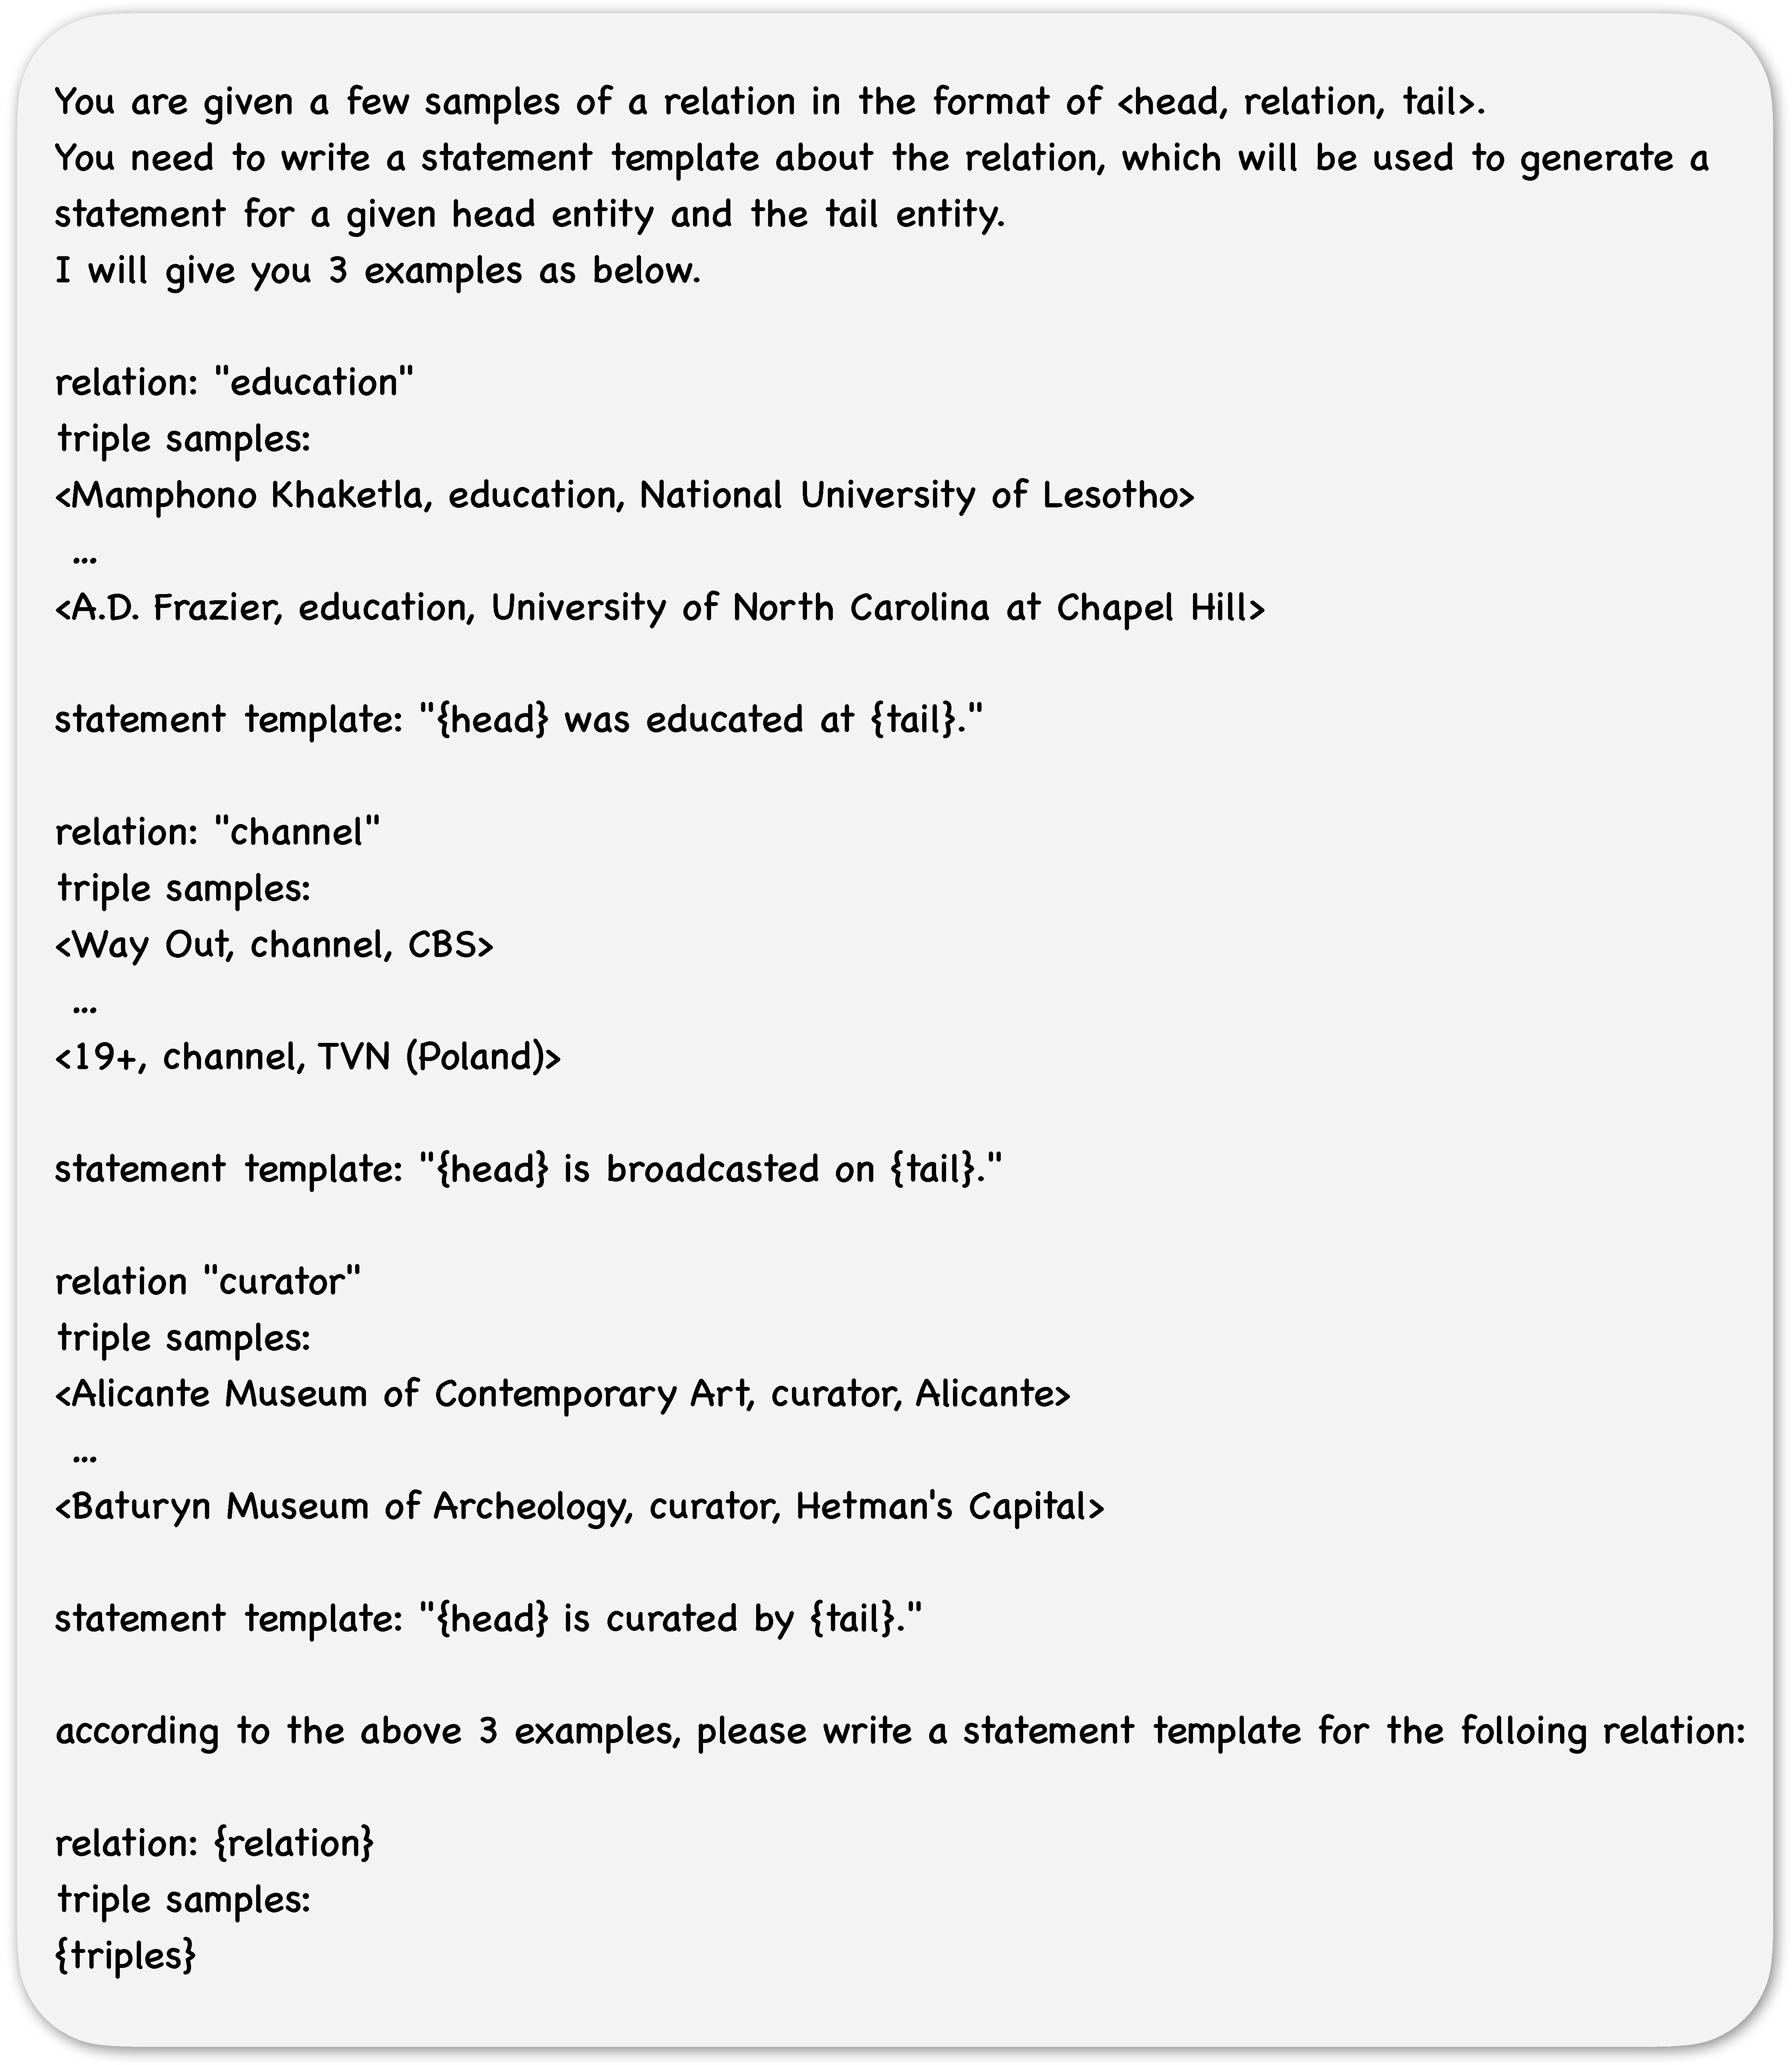
\includegraphics[width=4.5in]{submissions/Jing2024/figures/relation_template_prompt.pdf}
    \vspace{-3mm}
    \caption{The prompt to generate the relation template.}
    \label{fig:relation_template_prompt}
\end{figure}


\begin{table}[t]
    \centering\small\setlength{\tabcolsep}{0.2in}{
    \begin{tabular}{l|l|l}
    \toprule
    \textbf{Relation} & \textbf{Template} & \textbf{Count} \\
    \midrule

        birthPlace & The birthplace of \{head\} is \{tail\}. & 1,465,157 \\
    team & \{head\} is a part of the \{tail\} team. & 1,265,483 \\
    subdivision & The subdivision of \{head\} is \{tail\}. & 1,070,387 \\
    country &  \{head\} is from the country \{tail\}. & 766,844 \\
    starring &  \{head\} is a character in a movie or play \{tail\}". & 540,937 \\
    location & The location of \{head\} is \{tail\}. & 523,283 \\
    type & The type of \{head\} is \{tail\}. & 480,274 \\
    deathPlace & \{head\} passed away in \{tail\}. & 435,869 \\
    timeZone & The time zone of \{head\} is \{tail\}. & 433,915 \\
    genre & The genre of \{head\} is \{tail\}. & 415,336 \\
    homepage & The homepage of \{head\} is \{tail\}. & 366,745 \\
    position & The position of \{head\} is \{tail\}. & 319,196 \\
    seeAlso & The related item to \{head\} under the  & 296,615 \\
    & $\;\hookrightarrow$label 'seeAlso' is \{tail\}. & \\
    writer & The writer of \{head\} is \{tail\}. & 249,017 \\
    almaMater & The alma mater of \{head\} is \{tail\}. & 217,533 \\
    occupation & The occupation of \{head\} is \{tail\}. & 200,615 \\
    award & The award won by \{head\} is \{tail\}. & 181,521 \\
    recordLabel & The record label associated with \{head\} is \{tail\}. & 178,657 \\
    party & The party that \{head\} is affiliated with is \{tail\}. & 170,931 \\
    producer & The producer of \{head\} is \{tail\}. & 169,628 \\
    formerTeam & \{head\} used to play for \{tail\} team. & 151,374 \\
    family & \{head\} belongs to the \{tail\} family. & 148,818 \\
  currentMember & The current member of \{head\} is \{tail\}. & 148,739 \\
    battle & \{head\} participated in the following battles: \{tail\}. & 148,188 \\
    nationality &  The nationality of {head} is {tail}. & 147,525 \\ 
    director & The director of \{head\} is \{tail\}. & 145,621 \\
    associatedBand & The band associated with \{head\} is \{tail\}. & 135,597 \\
    associatedMusical& The musical artist associated with \{head\}   & 135,582 
    \\$\;\hookrightarrow$ Artist &$\;\hookrightarrow$  in the music industry is \{tail\}. & \\
    class & The class of \{head\} is \{tail\}. & 127,837 \\
    order & The order of \{head\} is \{tail\}. & 123,626 \\
    \bottomrule
    \end{tabular}}
    \caption{Relations templates.}
\label{tab:relation_templates}
\end{table}
   



\paragraph{Relation templates}
We use the relation templates to create queries for evaluating the models.
These templates are first generated by GPT with Web API in a few-shot manner, then manually curated to ensure the quality of the templates. We refer to Figure \ref{fig:relation_template_prompt} for the prompt used
for generating the relation templates. The prompt is designed to ask the model to generate a query for a given relation type. The model is asked to generate a query that can be used to judge the factuality of the relation type. We then manually curate the generated templates to ensure the quality of the templates. 
We refer to Table \ref{tab:relation_templates} for the curated relation templates.  Due to the large number of relation types in the DBpedia knowledge graph, we only showcase a few relation templates in the table, these templates are the most common relation types in the knowledge graph, sorted by the number of triples associated with the relation type.
 We can see that the relation templates are comprehensive and cover a wide range of topics. This can be seen as a source of multiple-domain knowledge for evaluating the LLMs.



\paragraph{Data and Model}
 We download the DBpedia data dump from \href{https://www.dbpedia.org/}{https://www.dbpedia.org/}. We use the turtle format of the DBpedia knowledge graph. 
 We directly use the LLaMA 2 and Gemma from the Hugging Face model hub. The model cards are
 \href{https://huggingface.co/meta-llama/Llama-2-7b-chat-hf}{meta-llama/Llama-2-7b-chat-hf}, \href{https://huggingface.com/meta-llama/Llama-2-13b-chat-hf}{ meta-llama/Llama-2-13b-chat-hf}, \href{https://huggingface.co/meta-llama/Llama-2-70b-chat-hf}{meta-llama/Llama-2-70b-chat-hf}, \href{https://huggingface.co/gemma-team/gemma-2b-chat-hf}{gemma-team/gemma-2b-chat-hf}, and \href{https://huggingface.co/gemma-team/gemma-7b-chat-hf}{gemma-team/gemma-7b-chat-hf}. 
 





  

    
    


\begin{table}[t]
    \centering
    \begin{tabular}{l|p{4.7in}}
    \toprule
    \textbf{Model} & \textbf{Instruction} \\ \midrule
    LLaMA 2 &   Below is an instruction that describes a task, paired with an input that provides further context. Write a response that appropriately completes the request.\textbackslash n\textbackslash n \#\#\# Instruction:\textbackslash n You are given a statement. You are asked to judge whether the statement is true or false. Answer 'Yes, the statement is true.' if you know the statement is true. Answer 'No, the statement is false.' if you know the statement is false. Otherwise, answer 'I don't know.'\textbackslash n\textbackslash n\#\#\# Input: {\bf Input} \textbackslash n\textbackslash n\#\#\# Response:\textbackslash n\textbackslash n 
                \\ \hline
    
    Gemma & start\_of\_turn\textgreater user  Below is an instruction that describes a task, paired with an input that provides further context. Write a response that appropriately completes the request.\textbackslash n\textbackslash n\#\#\# Instruction:\textbackslash n You are given a statement. You are asked to judge whether the statement is true or false. Answer 'Yes, the statement is true.' if you know the statement is true. Answer 'No, the statement is false.' if you know the statement is false. Otherwise, answer 'I don't know.'\textbackslash n\textbackslash n\#\#\# Input: {\bf Input} \textless end\_of\_turn\textgreater\textless start\_of\_turn\textgreater model\textbackslash n\textbackslash n The answer is " \\
    
    \bottomrule
    \end{tabular}
    \caption{Instruction used for creating queries.} %
    \label{tab:instruction} %
\end{table}


\paragraph{Instruction used for the LLaMA and Gemma models}
We report the instructions used for creating queries for the LLaMA and Gemma models. The instruction is designed to ask the model to judge whether the statement is true or false. We refer to Table \ref{tab:instruction} for the instruction used for creating queries. We use the same instruction for both the LLaMA and Gemma models with little modification to adjust the model's instruction format. With this instruction, the most frequent responses of LLMs are \textit{Yes, the statement is true}, \textit{No, the statement is false}, and \textit{I don't know}, with some variations on the suffix, mainly explaining the reason for the answer. This is what we expect from the LLMs when using a judge model (or the first-token logit as well), since the judge model doesn't use the LLM's response, but the hidden state of the LLM, which makes the consistency of the response format important. 


\subsection{Language Setting}

\xzrevision{As a framework, \GraphEval{} is not constrained by language, as long as the input is in the form of a knowledge graph. However, we did not conduct experiments on multilingual or cross-lingual datasets in the current work. Current experiments are conducted on English knowledge graphs.}
